No presente capítulo são descritos os detalhes do método para verificação de CIs proposto. Em seguida, é apresentada uma discussão acerca dos trabalhos relacionados com esta proposta. Por fim, é exposto o plano de trabalhos com as atividade planejadas ao longo deste curso.

\section{Método proposto}

Esta pesquisa propõe um método para verificação formal para detecção de vulnerabilidades em CIs escritos em Solidity na fase de pré-implementação. Especificamente, pretende-se detectar as vulnerabilidades de reentrância, \textit{delegatecall injection} e contrato suicida. Para isso, foi escolhida a técnica de \textit{model checking}, um método formal para verificação de sistemas de transição de estados que realiza uma pesquisa exaustiva sobre todo o espaço de estados do sistema para verificar se, conforme o modelo, o sistema age de acordo com propriedades predefinidas referentes à requerimentos de segurança e vivacidade do sistema.

Para isso, o código em Solidity deve ser convertido para algum formalismo baseado em estados que seja compatível com alguma ferramenta de verificação formal baseada em \textit{model checking}, como NuSMV~\footnote{\url{https://nusmv.fbk.eu/}}, nuXmv~\footnote{\url{https://nuxmv.fbk.eu/}}, SPIN~\footnote{\url{http://spinroot.com/}}, ou outra. Como as vulnerabilidades de reentrância e \textit{delegatecall injection} acontecem a partir da interação entre contratos (i.e., o contrato explorado e o contrato atacante), então o modelo de estados utilizado deve permitir a modelagem de relações ``intercontratuais''.

%Obs: dos \textit{model checkers} o nuXmv realiza o \textit{model checking} simbólico de sistemas de estados finito (ou infinitos) síncronos.

No \textit{model checking} as propriedades do sistema são especificadas por meio de fórmulas descritas em lógicas temporais LTL e CTL, ou alguma variação destas, como exposto nas Seções~\ref{tex:fund:metodos-formais} e~\ref{tex:fund:logicas-temporais}. Essas fórmulas são compostas por operadores temporais, quantificadores e elementos da lógica proposicional, técnicas que geralmente não são dominadas por desenvolvedores. Então, para facilitar a definição das propriedades, pretende-se desenvolver um modelo para descrição mais legível e mais próxima da linguagem natural, das propriedades que representem as vulnerabilidades abordadas. Vale destacar que, além das vulnerabilidades que são foco deste método de verificação, também será possível a inserção de qualquer propriedade relativa aos requisitos do CI, que ficará à critério do usuário. Este último ponto trata-se de algo que é intrínseco do \textit{model checking}, e que já está inerentemente incluso nos \textit{model checkers} existentes. Desta forma, também será possível a detecção de violações de propriedades funcionais.

No \textit{model checking}, quando o modelo não satisfaz uma propriedade, então é detectada uma violação, e um contraexemplo é fornecido para descrever o caminho de execução até a violação. No caso das vulnerabilidades alvos desta pesquisa, a violação de uma propriedade indica a presença desta vulnerabilidade.

Para implementar a proposta, será desenvolvido um framework que integre as seguintes atividades: inclusão do código fonte em Solidity; conversão do código para o modelo de estados; exibição do modelo obtido; inserção das propriedades e seleção das vulnerabilidades a serem verificadas; conversão das propriedades e vulnerabilidades para a fórmula em lógica temporal; verificação sobre o modelo de estados do contrato por meio do \textit{model checking}; e exibição dos resultados. Na inclusão do código fonte, mais de um arquivo pode ser inserido, já que o método proposto deve permitir a verificação considerando relações intercontratuais. Neste caso, devem ser indicadas manualmente pelo usuário as operações nas quais ocorre uma chamada externa à outro contrato. Desta forma, é obtido o diagrama de fluxo de interação entre os CIs, essencial para obtenção do modelo de transição de estados dos CIs. Uma vez fornecidos o código fonte e o diagrama de fluxo de interação dos CIs, é realizada a conversão automática para o modelo de transição de estados, que pode ser visualizado pelo usuário. Em seguida, as vulnerabilidades alvos da verificação são selecionadas, e, opcionalmente, outras propriedades também podem ser especificadas, e, adiante, são convertidas em fórmulas lógicas temporais. Enfim, o processo automático de \textit{model checking} pode ser iniciado. Encerrada a verificação, os resultados para cada vulnerabilidade e propriedade são exibidos. Em caso de detecção de uma vulnerabilidade ou violação de alguma propriedade, um contraexemplo é fornecido, indicando o caminho de execução resultante para cada vulnerabilidade detectada ou propriedade violada, assim como o fragmento de código responsável pela vulnerabilidade ou violação. O fluxo de trabalho do framework é ilustrado na Figura~\ref{fig:framework}. Nesta proposta, os únicos procedimento manuais necessários são a inserção das propriedades, e, quando for o caso, a descrição do diagrama de fluxo de interação dos contratos.

\begin{figure}[!htb]
 \caption{Fluxo de trabalho do framework proposto.}
 \label{fig:framework}
 \centering
 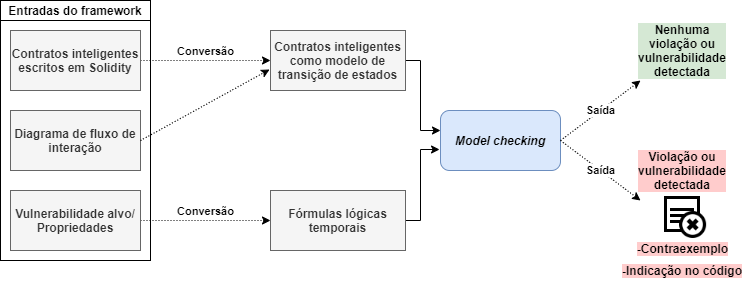
\includegraphics[scale=0.6]{figuras/framework.png}
 \fautor
\end{figure}

Como validação da proposta, será realizado experimento sobre um conjunto de contratos com vulnerabilidades já conhecidas, para, assim, poder avaliar a eficácia e acurácia da verificação, e outros aspectos como performance e a eficiência do framework proposto (i.e., consumo de memória, processamento, e tempo de execução). Além disso, também deve ser aplicado ao menos um estudo de caso para tratar de propriedades funcionais relativas aos requisitos do CI.

%% ver da onde vai tirar esses contratos, em uma daquelas páginas com vulnerabilidades 

\section{Trabalhos relacionados}

Esta seção tem o propósito de discutir a respeito das propostas encontradas na literatura para verificação de CIs baseadas em \textit{model checking}. Para coleta dos trabalhos, foi aproveitado o levantamento bibliográfico feito no MS desenvolvido na Seção~\ref{tex:rev:ms}, no qual os estudos selecionados foram classificados de acordo com a abordagem de verificação empregada. Nesta seção, são discutidos alguns dos estudos que propõem a abordagem de \textit{model checking}. 

Os trabalhos de~\citeonline{mavridou2019verisolid-103} e~\citeonline{nelaturu2020verified-101} são os primeiros a serem discutidos, e são os que possuem maior semelhança com o método proposto na presente pesquisa. No primeiro, que é um dos mais citados sobre o assunto, foi desenvolvido o framework VeriSolid, que permite a modelagem gráfica de CIs por meio de uma \sigla{MEF}{máquina de estados finito} que estende a semântica operacional da linguagem Solidity utilizada no framework FSolidM~\cite{mavridou2018tool-95}. Assim, o comportamento do contrato pode ser analisado com um alto nível de abstração, e então o código Solidity é gerado automaticamente a partir da MEF construída. Baseado na MEF obtida, pode-se definir propriedades de segurança e vivacidade para serem verificadas, porém, nenhuma vulnerabilidade específica foi abordada. Por meio da construção da MEF, diversos problemas são evitados, pois o código gerado do modelo é construído seguindo boas práticas de programação, como as recomendadas pela ConsenSys Diligence~\cite{consensys2021bestpractices}. No trabalho de cite~\citeonline{nelaturu2020verified-101} é proposta uma extensão da VeriSolid, na qual os contratos em Solidity são automaticamente convertidos para uma MEF que é incrementada com um diagrama de implementação, o qual consiste em informações relacionadas à relação entre múltiplos contratos. Além disso, também é acrescentado um módulo que realiza a implantação automática dos CIs gerados a partir da MEF. Nesse estudo, as vulnerabilidades de reentrância e de exceções não tratadas são prevenidas na própria construção da MEF, e as vulnerabilidades de endereço curto, contrato suicida e bloqueio de Ether são verificadas durante a modelagem ou na implantação do contrato. 

O framework desenvolvido por ~\citeonline{mavridou2019verisolid-103} e aperfeiçoado por~\citeonline{nelaturu2020verified-101} representa um dos maiores avanços na aplicação do \textit{model checking} para verificação de CIs, pois não exige que o usuário possua experiência com métodos formais, tanto para modelagem, quanto para definição das propriedades, a qual é feita com descrições em linguagem natural. Uma das lacunas deixadas por~\citeonline{nelaturu2020verified-101} é que, para prevenir a reentrância, não é permitido que funções sejam chamadas externamente (e.g., por meio de uma função \textit{fallback}) antes da finalização da transição atual, o que evita a recursividade de chamadas, porém, são desconsiderados casos em que uma função \textit{fallback} é utilizada sem representar necessariamente uma vulnerabilidade. Na estratégia proposta por esta pesquisa, pretende-se tratar estes casos, e também incluir a verificação da vulnerabilidade \textit{delegatecall injection}, explorada no ataque à \textit{Parity Wallet}, mencionado na Seção~\ref{tex:fund:ethereum:vuln-ataques}. 

\citeonline{bai2018formal-41} também propõem a modelagem do CI como uma MEF, codificada diretamente em PROMELA, a linguagem de entrada do \textit{model checker} SPIN~\footnote{\url{http://spinroot.com/}}. Entretanto, não é realizada nenhuma equivalência com o código fonte em Solidity, que sequer é retratado na abordagem proposta. O principal problema disso é que, representar os elementos de um CI diretamente em alguma outra linguagem ou formalismo que não sejam próprios para programação de CIs, não assegura que as propriedades e vulnerabilidades verificadas serão evitadas na eventual escrita do código em Solidity (ou em outra linguagem de programação aceita na Ethereum). O mesmo problema também ocorre em~\citeonline{liu2019formal-42}, ~\citeonline{madl2019formal-46}, ~\citeonline{he2020modeling-60}, ~\citeonline{kongmanee2019securing-78}, ~\citeonline{shishkin2019debugging-22} e~\citeonline{abdellatif2018formal-44}. Na estratégia proposta nesta pesquisa, essa limitação é evitada, pois pressupõe que as vulnerabilidades e violações detectadas serão apontadas no código para correção.

No estudo de~\citeonline{wang2019detecting-nondeterministic-26} é proposta a ferramenta de verificação NPChecker, cuja estratégia de modelagem e detecção de violação de propriedades nos contratos é feita com o objetivo de expor o não-determinismo da execução das transações na Ethereum como a raiz de vulnerabilidades relacionadas à \textit{bugs} de pagamentos e transferências. Especificamente, são tratadas as vulnerabilidades de reentrância, dependência de ordem de transação e falha de chamada externa (também conhecida como chamada externa não verificada). Diferente do que é proposto na presente pesquisa, em~\citeonline{wang2019detecting-nondeterministic-26} é empregada uma estratégia totalmente automatizada, na qual não é necessário analisar individualmente cada contrato, o que favorece a aplicação de experimentos em larga escala, porém, por outro lado, afeta a acurácia da verificação e introduz falsos positivos.

%Nos trabalhos ~\cite{osterland2020model-58, he2020modeling-60, chen2020gaschecker-50, chen2020gaschecker-50} não são consideradas relações inter-contratuais.

\subsection{Conclusão}

Como exposto na Seção~\ref{tex:rev:ms:publicacao}, o \textit{model checking} é um dos métodos de verificação mais adotados em pesquisas recentes que abordam a verificação de CIs. Contudo, ainda há diversas limitações presentes na maior parte desses trabalhos. Um dos entraves para a adoção do \textit{model checking} e outros métodos formais para verificação de CIs é a realização de procedimentos manuais que exigem conhecimento específico sobre os métodos formais empregados. Os trabalhos levantados nesta pesquisa que apresentam tal limitação são citados na Seção~\ref{tex:rev:ms:publicacao}. 

Ademais, poucos trabalhos consideram relações intercontratuais para modelagem e verificação. Neste sentido, o trabalho de~\citeonline{nelaturu2020verified-101} apresentou um dos maiores avanços nessa área, pois além de tratar as relações entre múltiplos contratos, também evita a necessidade de conhecimento sobre os métodos formais utilizados, já que os procedimentos de tradução do código fonte, obtenção do modelo, e análise e interpretação dos resultados são realizados automaticamente pelo framework. Além disso, apesar da especificação das propriedades ser feita manualmente, esse procedimento é simplificado por normas para especificação em linguagem natural. 

Por meio do estratégia de verificação de CIs proposta neste trabalho, pretende-se usufruir dos avanços já realizados, e estender algumas funcionalidades como o tratamento especial das funções \textit{fallback} para verificação da vulnerabilidade de reentrância, a detecção da vulnerabilidade \textit{delegatecall injection} e a indicação do fragmento do código fonte que ocasionar o problema detectado.

\section{Plano de trabalho} \label{cap:cronograma}

Na plano de trabalho exposto na Tabela~\ref{tab:cronograma}, são expostas as atividades já desenvolvidas até então, e também as que serão realizadas até a defesa da dissertação para conclusão do mestrado. 

\begin{table}[!ht]%[H]
\centering
\fontsize{10pt}{10pt}\selectfont
%\addtolength{\tabcolsep}{-4pt}
\caption{Plano de trabalho das atividades do mestrado}
\label{tab:cronograma}
\begin{tabular}{|l|l|l|l|l|l|l|l|l|l|l|l|l|l|} 
\hline
                                         & \multicolumn{5}{c|}{\textbf{2020}}                                                                                                                                                                    & \multicolumn{6}{c|}{\textbf{2021}}                                                                                                                                                                                                            & \multicolumn{2}{c|}{\textbf{2022}}                                             \\ 
\cline{2-14}
\textbf{\textbf{Atividade}}              & \begin{sideways}Mar-Abr\end{sideways} & \begin{sideways}Mai-Jun\end{sideways} & \begin{sideways}Jul-Ago\end{sideways} & \begin{sideways}Set-Out\end{sideways} & \begin{sideways}Nov-Dez\end{sideways} & \begin{sideways}Jan-Fev\end{sideways} & \begin{sideways}Mar-Abr\end{sideways} & \begin{sideways}Mai-Jun\end{sideways} & \begin{sideways}Jul-Ago\end{sideways} & \begin{sideways}Set-Out\end{sideways} & \begin{sideways}Nov-Dez\end{sideways} & \begin{sideways}Jan-Fev\end{sideways} & \begin{sideways}Mar-Abr\end{sideways}  \\ 
\hline
Obtenção dos créditos obrigatórios       & {\cellcolor[rgb]{0.396,0.396,0.396}}  & {\cellcolor[rgb]{0.396,0.396,0.396}}  & {\cellcolor[rgb]{0.396,0.396,0.396}}  & {\cellcolor[rgb]{0.396,0.396,0.396}}  & {\cellcolor[rgb]{0.396,0.396,0.396}}  &                                       &                                       &                                       &                                       &                                       &                                       &                                       &                                        \\ 
\hline
Estudo da tecnologia blockchain          &                                       &                                       & {\cellcolor[rgb]{0.396,0.396,0.396}}  & {\cellcolor[rgb]{0.396,0.396,0.396}}  & {\cellcolor[rgb]{0.396,0.396,0.396}}  &                                       &                                       &                                       &                                       &                                       &                                       &                                       &                                        \\ 
\hline
Estudo da blockchain Ethereum e dos CIs  &                                       &                                       & {\cellcolor[rgb]{0.396,0.396,0.396}}  & {\cellcolor[rgb]{0.396,0.396,0.396}}  & {\cellcolor[rgb]{0.396,0.396,0.396}}  & {\cellcolor[rgb]{0.396,0.396,0.396}}  & {\cellcolor[rgb]{0.396,0.396,0.396}}  & {\cellcolor[rgb]{0.396,0.396,0.396}}  & {\cellcolor[rgb]{0.396,0.396,0.396}}  &                                       &                                       &                                       &                                        \\ 
\hline
Estudo dos métodos de verificação de CIs &                                       &                                       &                                       & {\cellcolor[rgb]{0.396,0.396,0.396}}  & {\cellcolor[rgb]{0.396,0.396,0.396}}  & {\cellcolor[rgb]{0.396,0.396,0.396}}  & {\cellcolor[rgb]{0.396,0.396,0.396}}  & {\cellcolor[rgb]{0.396,0.396,0.396}}  & {\cellcolor[rgb]{0.396,0.396,0.396}}  &                                       &                                       &                                       &                                        \\ 
\hline
Realização do MS                         &                                       &                                       &                                       & {\cellcolor[rgb]{0.396,0.396,0.396}}  & {\cellcolor[rgb]{0.396,0.396,0.396}}  & {\cellcolor[rgb]{0.396,0.396,0.396}}  & {\cellcolor[rgb]{0.396,0.396,0.396}}  & {\cellcolor[rgb]{0.396,0.396,0.396}}  &                                       &                                       &                                       &                                       &                                        \\ 
\hline
Preparação da qualificação               &                                       &                                       &                                       &                                       &                                       & {\cellcolor[rgb]{0.396,0.396,0.396}}  & {\cellcolor[rgb]{0.396,0.396,0.396}}  & {\cellcolor[rgb]{0.396,0.396,0.396}}  &                                       &                                       &                                       &                                       &                                        \\ 
\hline
Implementação do método proposto         &                                       &                                       &                                       &                                       &                                       &                                       &                                       &                                       & {\cellcolor[rgb]{0.396,0.396,0.396}}  & {\cellcolor[rgb]{0.396,0.396,0.396}}  &                                       &                                       &                                        \\ 
\hline
Avaliação experimental                   &                                       &                                       &                                       &                                       &                                       &                                       &                                       &                                       &                                       & {\cellcolor[rgb]{0.396,0.396,0.396}}  & {\cellcolor[rgb]{0.396,0.396,0.396}}  &                                       &                                        \\ 
\hline
Redação da dissertação                   &                                       &                                       &                                       &                                       &                                       &                                       &                                       &                                       &                                       & {\cellcolor[rgb]{0.396,0.396,0.396}}  & {\cellcolor[rgb]{0.396,0.396,0.396}}  & {\cellcolor[rgb]{0.396,0.396,0.396}}  &                                        \\ 
\hline
Defesa do mestrado                       &                                       &                                       &                                       &                                       &                                       &                                       &                                       &                                       &                                       &                                       &                                       &                                       & {\cellcolor[rgb]{0.396,0.396,0.396}}   \\
\hline
\end{tabular}
\end{table}